\documentclass[conference]{IEEEtran}
\usepackage{amsmath,amssymb}
\usepackage{booktabs}
\usepackage{graphicx}
\usepackage{array}
\usepackage[numbers,sort&compress]{natbib}
\usepackage{microtype}
\usepackage{xcolor}
\usepackage[hidelinks,hypertexnames=false]{hyperref}
\usepackage{enumitem}
\usepackage{float}

\newcommand{\todo}[1]{\textcolor{red}{[TODO: #1]}}

% Headline numbers, defined once so prose and tables cannot drift.
\newcommand{\maptest}{0.976}
\newcommand{\mapstd}{0.003}
\newcommand{\fps}{1.165}
\newcommand{\fpn}{7.266}
\newcommand{\fpct}{6.2}
\newcommand{\manifestsum}{748322d6}

\title{Not the Metric You Report:\\
Leakage-Audited Landmine Surface Detection,\\
and Why mAP$_{50}$ Cannot Choose an Operating Point}

\author{\IEEEauthorblockN{Anonymous Authors}%
\IEEEauthorblockA{Preprint. Under review.}}

\begin{document}
\maketitle

\begin{abstract}
Detection benchmarks in aerial and remote-sensing settings are usually ranked by
mean average precision (mAP). We show that on a small, single-class landmine
surface-indicator dataset this ranking is uninformative for deployment: a
3.0\,M-parameter detector and an 11.1\,M-parameter detector differ by less than
the seed-to-seed spread in test mAP$_{50}$ ($0.979$ vs.\ $0.977 \pm 0.003$), yet their
recall-first operating points differ by a factor of $4.3$ in false positives per
image ($6.50$ vs.\ $1.51$). We argue that the meaningful object of study is the
operating point, not the summary curve, and we build the evaluation protocol
around that claim.

The study rests on two methodological contributions that require no new
architecture. First, we audit a widely reused landmine image corpus and find that
its published split leaks: $76$ Roboflow base-name groups span splits and
$63.8\%$ of evaluation images have a near-duplicate in training, consistent with
augmentation applied before splitting. We rebuild the split group-wise, apply a
two-method leak filter (perceptual hash plus pixel MSE) with manual review of
every candidate, and remove $30$ evaluation images. The frozen manifest
(3{,}907 / 181 / 189 images; digest \texttt{\manifestsum\ldots}) contains no
exact duplicate, no base-key collision, and no confirmed near-duplicate leak.

Second, we measure what the leak was worth. A detector trained on the leaky split
scores $0.994$ mAP$_{50}$ on the full clean test set against $0.974$ for a
clean-trained model, but on the $49$ contamination-free test images the two are
tied ($0.995$ vs.\ $0.995$). The apparent inflation is therefore contamination,
not capability---and it is small, a negative result we report rather than bury.

We then evaluate a MobileNetV3-Large second stage over detector crops on three
detector seeds. The two-stage arm improves precision over a recall-matched
single-stage baseline at two of three seeds ($\Delta P = +0.128$ and $+0.144$,
bootstrap intervals excluding zero) but fails at the third
($\Delta P = -0.037$, interval $[-0.077, +0.013]$). Under a max-$F_2$ rule a
val-tuned single-stage threshold beats the two-stage pipeline outright
($P = 0.976$ vs.\ $0.945$). We report the effect as detector-dependent rather
than architectural, and we identify the mechanism: the two-stage gain comes from
rescuing seeds whose val-selected threshold transferred poorly, not from better
localisation. Grad-CAM confirms that the detector's evidence lies on the objects
(median $58\times$ energy enrichment over chance) and that the second stage adds
almost no spatial evidence of its own ($1.82\times$ for the image-level baseline,
$2.13\times$ for crops)---a caution against reading a classifier's accuracy as
reasoning. All experiments were run on one 8\,GB laptop GPU within a
$\sim$30\,h budget; we state explicitly what that budget forbade.
\end{abstract}


\begin{IEEEkeywords}
landmine detection, object detection, dataset leakage, operating point,
evaluation protocol, YOLOv8
\end{IEEEkeywords}

\section{Introduction}
\label{sec:intro}

A landmine detector that is evaluated with mean average precision is being asked
the wrong question. Mean average precision integrates performance over every
confidence threshold and every recall level, then reduces the result to one
number. A demining team does not operate a curve; it operates one threshold, on
one day, with one tolerance for false alarms. Two systems can share a curve and
behave completely differently at the threshold that will actually be used. This
paper is an extended argument, with measurements, that the operating point---and
not the summary curve---is the object that should be reported, and that the
usually unglamorous work of auditing the split is what makes any such comparison
believable.

We study single-class detection of \emph{surface} landmine indicators from
downward-looking aerial imagery. The scope limitation is physical and we state it
first: a visible-light or colour camera cannot see a buried object. What it can
see is a mine lying on the surface, a partially exposed casing, or a surface
marker. Claims in this paper are therefore claims about visible surface objects,
not about buried ordnance, and nothing here is a field-validated clearance
system. The task is nonetheless a useful stress test for detection methodology,
because the class is rare, the imagery is heterogeneous, and the published data
reuse is heavy.

\paragraph{What we found.} Three results organise the paper.

\begin{enumerate}[leftmargin=1.2em,itemsep=2pt]
\item \textbf{The split leaks, and the leak is measurable.} The combined
landmine corpus contains $76$ filename groups (Roboflow base names) that span
train and evaluation splits, and $63.8\%$ of validation and test images have a
perceptual-hash neighbour in training. This is the signature of augmentation
applied before splitting: the same scene, re-exported, lands on both sides of the
boundary. After rebuilding the split group-wise and filtering twice, $30$
evaluation images are removed as true leaks. A detector trained on the leaky
split scores $0.994$ mAP$_{50}$ on the full clean test set, against $0.974$ for a
clean-trained detector. On the $49$ test images that are contamination-free for
both, the two are tied at $0.995$ and $0.995$. The leak inflated the number, but
by less than the folklore predicts---a negative result, and one that would have
been invisible without the contamination-free subset.

\item \textbf{mAP$_{50}$ does not settle the deployment question.} A YOLOv8s
detector over three seeds reaches $0.977 \pm 0.003$ test mAP$_{50}$; the one
available YOLOv8n seed reaches $0.979$. Although the n point is slightly higher
on test, validation mAP favors s ($0.954$ vs. $0.932$), and n has no seed
interval. At the recall-first operating point chosen on validation, the observed
n checkpoint produces $6.50$ false positives per image against $1.51$ for s.
We present this as a case study in threshold transfer and operating-point
reporting, not as a reliable model-ranking reversal.

\item \textbf{The two-stage gain is detector-dependent, and we can say why.} A
MobileNetV3-Large classifier over detector crops improves precision over a
recall-matched single-stage baseline at two of three detector seeds
($\Delta P = +0.128$ and $+0.144$, paired bootstrap intervals excluding zero).
At the third seed it is \emph{worse} ($\Delta P = -0.037$, interval
$[-0.077, +0.013]$). Under a max-$F_2$ rule, a single confidence threshold tuned
on validation beats the two-stage pipeline outright ($P = 0.976$ vs.\ $0.945$).
The pattern is consistent with the classifier helping when the validation-selected
detector threshold transfers poorly to test, but three seeds do not identify that
mechanism. Where the baseline threshold transfers well, the second stage has
nothing to add. Reporting a three-seed mean of $0.879 \pm 0.018$ would have hidden
this entirely; we report the per-seed structure instead.
\end{enumerate}

\paragraph{Why this is worth publishing.} None of the three findings required a
new architecture, a large GPU, or a new dataset. They required (i) reconstructing
the split from scratch, (ii) refusing to average over seeds when the seeds
disagree structurally, and (iii) measuring at the operating point rather than at
the summary. The total compute was one 8\,GB laptop GPU and roughly $30$ hours.
We think this is a realistic and under-reported budget for applied detection
work, and we document what it forbade (Section~\ref{sec:limitations}) rather than
implying broader coverage.

\paragraph{Contributions.}
\begin{itemize}[leftmargin=1.2em,itemsep=2pt]
\item A reproducible leakage audit of a publicly derived landmine corpus: an
operational leak definition, a two-method filter with a manually validated MSE
cut, a frozen manifest, and an accounting of all $30$ removals
(Section~\ref{sec:audit}).
\item A direct leaky-versus-clean comparison on a contamination-free subset,
including the unfavourable result that the mAP difference on a small
contamination-free subset is small, while threshold-matched operating-point
effects remain unmeasured
(Section~\ref{sec:leakvalue}).
\item An operating-point evaluation protocol---thresholds chosen on validation
only, applied once to test, with paired image bootstrap and source-cluster
intervals---and a case study showing why a single mAP-based ranking can be
insufficient
(Section~\ref{sec:results}).
\item A per-seed analysis of a two-stage detector-plus-classifier pipeline that
localises a failure rather than averaging it away, together with a max-$F_2$
analysis showing when the second stage is not worth its cost
(Section~\ref{sec:twostage}).
\item A Grad-CAM audit used as a sanity check on evidence, with an explicit
separation between attribution and correctness, showing that the image-level
classifier's accuracy is not accompanied by object-level evidence
(Section~\ref{sec:gradcam}).
\end{itemize}

Section~\ref{sec:related} positions the work; Section~\ref{sec:data} describes the
corpus and its provenance; Section~\ref{sec:audit} the audit;
Sections~\ref{sec:method}--\ref{sec:protocol} the models and protocol;
Section~\ref{sec:results} the results; Sections~\ref{sec:discussion}--\ref{sec:ethics}
discussion, limitations and ethics. Code, weights, tables and the frozen split
manifest accompany the paper (Section~\ref{sec:availability}).

\section{Related Work}
\label{sec:related}

\paragraph{Landmine and UXO detection.} The physical sensing literature is
large and predates deep learning by decades: metal detectors, ground-penetrating
radar, infrared and multispectral sensing, and combinations thereof
\citep{siegel2002landmine,kasban2010comparative}. What matters for this paper is
a distinction that the computer-vision literature often blurs. Subsurface sensing
asks whether a buried object is present; visible-band aerial imaging asks whether
a surface object or marker is visible. The two tasks have different base rates,
different failure modes, and different false-alarm costs. We therefore restrict
every claim to the visible-surface task and treat buried-object performance as
out of scope rather than as a gap to be estimated. The humanitarian scale of the
problem is documented annually by the Landmine Monitor \citep{icbl2023landmine};
we mention it to motivate careful evaluation, not to claim operational utility.

\paragraph{Detectors.} The YOLO family \citep{redmon2018yolov3,jocher2023ultralytics}
remains the default for small-object aerial detection because of its latency at
moderate resolution. Alternatives include anchor-free and transformer-based
detectors \citep{tian2019fcos,carion2020detr,zhao2024rtdetr} and two-stage
region proposals \citep{ren2015faster}, with focal loss
\citep{lin2017focal} addressing foreground imbalance. Our contribution is not a
detector. We deliberately use the most standard available baseline, because the
point is that evaluation choices dominate architecture choices at this scale. The
lightweight classifier in our second stage is MobileNetV3-Large
\citep{howard2019mobilenetv3} ($3{,}119{,}535$ parameters, torchvision
\texttt{mobilenet\_v3\_large} with ImageNet weights), chosen for cost rather than
novelty.

\paragraph{Leakage and reproducibility.} That machine-learning results can be
inflated by information leaking across train and evaluation splits is now well
documented, both as a general methodological failure
\citep{kapoor2023leakage,kapoor2024reforms,roberts2021pitfalls} and in specific
benchmarks \citep{recht2019imagenet,barz2020train}. The canonical defence is
group-aware splitting, so that no group---scene, patient, site, or source
document---spans the boundary; and once the split is fixed, the estimator used to
turn it into a number is itself a choice, since cross-validation and bootstrap
schemes of the same data do not agree with each other \citep{kohavi1995study}. In
image corpora, groups
must be recovered from pixels when filenames are unreliable: perceptual hashing
\citep{zauner2010phash} proposes near-duplicate candidates, and a pixel-space
distance such as MSE or SSIM \citep{wang2004ssim} separates true re-exports from
terrain-texture coincidences. Our audit follows exactly this two-stage pattern,
and we report the threshold at which the two methods disagree. Publicly shared
detection datasets frequently originate as re-exports of the same source
collection, which is why base-key collisions matter independently of pixels.

\paragraph{Evaluation beyond mAP.} The mismatch between average precision and
deployed behaviour is an old observation in detection. \citet{hoiem2012diagnosing}
argued for error diagnosis over single scores; \citet{dollar2012pedestrian}
popularised log-average miss rate at a fixed false-positive-per-image budget
precisely because average precision hides the low-false-alarm regime. Our
protocol adopts false-positives-per-image at a recall-first operating point as the
primary quantity, and reports mAP only as a secondary, comparable-to-the-literature
number. We also follow the recommendation to report intervals rather than point
estimates: paired image bootstrap for comparisons on the same images
\citep{efron1993bootstrap}, and source-cluster resampling where the effective
sample size is the number of acquisition sources, not the number of images.
Agreement statistics use Cohen's $\kappa$ \citep{cohen1960kappa} for image-level
decisions. Dataset and model documentation follow the datasheet and model-card
conventions \citep{gebru2021datasheets,mitchell2019modelcards}.

\paragraph{Attribution methods.} Grad-CAM \citep{selvaraju2017gradcam} and its
variants \citep{chattopadhyay2018gradcampp} are widely used to argue that a model
``looks at the right thing''. The evidence that saliency maps can be insensitive
to model parameters \citep{adebayo2018sanity}, and that deletion-style tests are
the appropriate falsification \citep{samek2017evaluating}, means attribution
should be treated as a diagnostic and never as proof of correctness. The
Clever Hans literature \citep{lapuschkin2019unmasking} is the cautionary case: a
classifier can be accurate for the wrong reason. We use Grad-CAM in that
falsification role only, and we report where it fails.

\section{Data}
\label{sec:data}

\subsection{Corpus and task}

The corpus pools five public Roboflow Universe landmine-detection exports,
identified here by source id: \texttt{ds0}, \texttt{ds1}, \texttt{May\_lwir},
\texttt{Jan\_lwir}, and a small derived set folded into \texttt{ds0}. Each image
carries one class, \texttt{landmine}, and axis-aligned boxes. There is no
mine-type label; the task is presence and localisation of a visible
mine-like object. Table~\ref{tab:data} gives the frozen split.

\begin{table*}[t]
\centering
\small
\caption{Frozen dataset \texttt{landmine\_combined\_v2}. ``neg'' counts images
with an empty label file (deliberate negatives), not missing labels; there are
zero missing labels. Manifest digest
\texttt{748322d6\ldots c80de}.}
\label{tab:data}
\begin{tabular}{lrrrr}
\toprule
split & images & instances & neg & sources \\
\midrule
train & 3{,}907 & 11{,}550 & 20 & Jan 100, May 776, ds0 2{,}589, ds1 442 \\
valid & 181 & 419 & 7 & Jan 42, ds0 138, ds1 1 \\
test & 189 & 253 & 5 & Jan 10, ds0 151, ds1 28 \\
\bottomrule
\end{tabular}
\end{table*}

The class is heavily imbalanced in the detection sense and, more importantly,
heterogeneous in acquisition. Table~\ref{tab:shift} shows the source/split shift
that dominates the results later. \texttt{Jan\_lwir} images average $7.7$ boxes
per test image; \texttt{ds0} and \texttt{ds1} average about one. A model that
learns ``many objects'' from \texttt{Jan} and applies it to \texttt{ds0} will
generate false positives by construction, and vice versa. This is not a nuisance
to be averaged away: it is the principal source of variance in the test set, and
we return to it in Section~\ref{sec:persource}.

\begin{table*}[t]
\centering
\small
\caption{Source and split composition. The test set is dominated by
\texttt{ds0} images (151 of 189) but by \texttt{Jan} boxes (77 of 253).}
\label{tab:shift}
\begin{tabular}{llrrrr}
\toprule
split/source & & images & boxes & boxes/img & empty rate \\
\midrule
test & Jan\_lwir & 10 & 77 & 7.70 & 0.00\% \\
test & ds0 & 151 & 148 & 0.98 & 1.99\% \\
test & ds1 & 28 & 28 & 1.00 & 7.14\% \\
\midrule
train & Jan\_lwir & 100 & 740 & 7.40 & 0.00\% \\
train & May\_lwir & 776 & 7{,}706 & 9.93 & 0.00\% \\
train & ds0 & 2{,}589 & 2{,}643 & 1.02 & 0.77\% \\
train & ds1 & 442 & 461 & 1.04 & 0.00\% \\
\midrule
valid & Jan\_lwir & 42 & 287 & 6.83 & 0.00\% \\
valid & ds0 & 138 & 131 & 0.95 & 5.07\% \\
valid & ds1 & 1 & 1 & 1.00 & 0.00\% \\
\bottomrule
\end{tabular}
\end{table*}

\subsection{Two content defects, disclosed}

\paragraph{The \texttt{lwir} files are not thermal.} Sources named
\texttt{May\_lwir} and \texttt{Jan\_lwir} suggest long-wave infrared imagery. They
are not. Mean HSV saturation on a $24$-image sample is $0.38$, against $0.25$ for
the \texttt{ds0} RGB reference, and the images carry visible marker pins. They are
colour RGB photographs. We keep them, because removing them would drop the only
multi-object source and make the task artificially easy, and we disclose the
consequence: a model could exploit marker pins as a shortcut. A twelve-crop zoom
check around test mines found no consistent marker, paint, or flag cue, but we
cannot rule out a subtler one, and we do not make thermal claims anywhere in this
paper.

\paragraph{Two test labels are objectively wrong.} Manual review identified two
test boxes that are not on mines: \texttt{ds0\_0801} annotates a tree trunk and
\texttt{ds0\_0883} annotates a fence. Both were confirmed independently by a
Grad-CAM energy of exactly zero (Section~\ref{sec:gradcam}). We remove them from
ground truth and report results both with and without the correction
(Table~\ref{tab:labelfix}). No training labels were found to be wrong, so no
retraining was performed.

\begin{table}[t]
\centering
\small
\caption{Effect of removing two objectively wrong test boxes (no retraining).
Intervals in the source artifact are unchanged; the shift is a ground-truth
correction, not a model change.}
\label{tab:labelfix}
\begin{tabular}{lccc}
\toprule
arm & metric & before & after \\
\midrule
C (two-stage) & box recall & 0.9644 & 0.9721 \\
C (two-stage) & image recall & 0.9891 & 1.0000 \\
C (two-stage) & FP/image & 0.153 & 0.153 \\
A (YOLO deploy) & box recall & 0.9763 & 0.9841 \\
B (YOLO matched) & box recall & 0.9723 & 0.9801 \\
\bottomrule
\end{tabular}
\end{table}

\subsection{Provenance and redistribution}

The source archives were obtained as public exports, but their licence terms were
not recorded at download time and the original project URLs are no longer
available to this project. We therefore do not redistribute any image, label file,
or crop. What is released is the split manifest with a SHA-256 digest, the
removed-leak list with reasons, the audit CSVs and montages, the trained weights,
and the code. Anyone holding the original archives can reconstruct the exact
splits byte-for-byte from the manifest. Full detail is in
\texttt{DATA\_PROVENANCE.md}; the weights carry the upstream Ultralytics AGPL-3.0
terms (Section~\ref{sec:availability}). We regard the missing licence record as a
defect of this study and state it rather than inferring a permissive licence.

\section{Leakage Audit}
\label{sec:audit}

\subsection{The original split fails}

The first audit pass over the pooled corpus returned a clear failure. Of the
evaluation images, $63.8\%$ had a training image within perceptual-hash Hamming
distance $2$, and $76$ Roboflow base names appeared in more than one split
(train$\cap$valid $37$, train$\cap$test $31$, valid$\cap$test $10$). A montage
of the base-name collisions shows the same physical scene, the same mine
placement, and different export bytes: these are re-exports, not distinct
photographs. The mechanism is augmentation before splitting, present in the
upstream generation scripts. The test split also contained zero negative images,
so false-alarm rate was undefined. We therefore discarded the split entirely
rather than attempting to patch it.

\subsection{Operational leak definition}

A validation or test image $x$ is a leak if any training image shares any of:

\begin{enumerate}[leftmargin=1.4em,itemsep=1pt]
\item the exact MD5 digest;
\item the Roboflow base key (filename with the \texttt{*.rf.<md5>.jpg} export
suffix stripped);
\item the same source id \emph{and} a 64-bit perceptual hash \citep{zauner2010phash}
within Hamming distance $2$ under all eight dihedral transforms, \emph{and} a
$32\times32$ RGB mean-squared error below $900$.
\end{enumerate}

Condition 3 is a conjunction for a reason. Perceptual hash alone over-fires on
repetitive terrain: grass and dirt produce Hamming collisions that are not the
same scene. The MSE term separates the two populations, and manual review sets
the cut. Every Hamming-$\le 2$ candidate---$146$ pairs across two rounds---was
rendered side by side and inspected. Confirmed same-scene pairs occurred at
$\mathrm{MSE} \le 817$; terrain-texture coincidences at
$\mathrm{MSE} \ge 958.6$. The gap is narrow but unambiguous on montage, and the
cut at $900$ sits inside it.

\subsection{Rebuilding and freezing}

Groups were formed from base key, capture session, and same-source hash edges,
yielding $1{,}048$ groups, then assigned whole to a split. Two filtering passes
removed $30$ evaluation images: $13$ at $\mathrm{MSE}\le 100$, then $17$ more at
$\mathrm{MSE}\le 900$, including a cross-folder duplicate
(\texttt{ds0\_0043}$\leftrightarrow$\texttt{ds1\_0043}). The split is
$19$ validation and $11$ test images lighter as a result. The residual $99$ of
$370$ evaluation images with a Hamming-$\le 2$ training neighbour all have
$\mathrm{MSE} \ge 958.6$ and were verified as texture false positives. True leak
rate: $0/370$.

\begin{table}[t]
\centering
\small
\caption{Leakage audit outcome for the frozen split. ``Residual candidates''
are Hamming-$\le2$ pairs rejected by the pixel-MSE test and manual review.}
\label{tab:audit}
\begin{tabular}{lr}
\toprule
quantity & value \\
\midrule
Images (train / valid / test) & 3{,}907 / 181 / 189 \\
Instances & 11{,}550 / 419 / 253 \\
Negatives & 20 / 7 / 5 \\
Exact cross-split duplicate groups & 0 \\
Base-key collisions (train-valid / train-test / valid-test) & 0 / 0 / 0 \\
Residual near-duplicate candidates & 99 (all MSE $\ge 958.6$) \\
Evaluation images removed as leaks & 30 (19 valid, 11 test) \\
Confirmed true leak rate & $0/370 = 0.0\%$ \\
Manifest SHA-256 & \texttt{748322d6\ldots c80de} \\
\bottomrule
\end{tabular}
\end{table}

\subsection{What the leak was worth}
\label{sec:leakvalue}

An audit is only useful if it changes something. We therefore trained a YOLOv8s
detector on the \emph{old} split (the ``leaky'' model) and compared it with the
clean-trained seed-0 detector on the clean test set. This is the natural
before/after experiment, and it has a trap: $140$ of $189$ clean test images
($74.1\%$) share a v2 group with an image the leaky model trained on. Scoring the
leaky model on the full test set therefore measures memorisation.

The results are in Table~\ref{tab:leaky}. On its own split the leaky model
reaches $0.970$ mAP$_{50}$, but that split has zero negatives, so false-positive
rate is undefined and the number cannot be compared with anything in this paper.
On the full clean test set it reaches $0.994$, comfortably above the clean
model's $0.974$. On the $49$ contamination-free images the two are tied:
$0.9950$ against $0.9947$ mAP$_{50}$, and $0.725$ against $0.701$ mAP$_{50\text{--}95}$.
The $49$-image subset is small and the comparison is therefore low-powered, but
the direction is unambiguous: the apparent $+0.020$ advantage is contamination,
and the honest estimate of the leak's effect on this corpus is close to zero.

\begin{table}[t]
\centering
\small
\caption{Leaky-versus-clean comparison. The leaky model's operating confidence
($0.065$) was chosen on the old validation split; the clean model's ($0.02$) on
the new one. P and FP/image are therefore not threshold-matched and mAP is the
fair column.}
\label{tab:leaky}
\begin{tabular}{llcccc}
\toprule
model & evaluation set & mAP$_{50}$ & mAP$_{50\text{--}95}$ & P & FP/img \\
\midrule
leaky v1 & v1 test (own split) & 0.9697 & 0.6436 & 0.834 & n/a (0 neg) \\
leaky v1 & v2 test, full (74.1\% contaminated) & 0.9940 & --- & 0.857 & 0.222 \\
clean v2 s0 & v2 test, full & 0.9741 & 0.6924 & 0.427 & 1.751 \\
\midrule
leaky v1 & v2 test, contamination-free ($n=49$) & 0.9950 & 0.7250 & 0.863 & 0.204 \\
clean v2 s0 & v2 test, contamination-free ($n=49$) & 0.9947 & 0.7010 & 0.354 & 2.347 \\
\bottomrule
\end{tabular}
\end{table}

This is a negative result and we treat it as one. The literature on leakage
\citep{kapoor2023leakage,recht2019imagenet} prepares one to expect a large
inflation. Here the clean and leaky models converge on the leak-free images, which
suggests that for this task the leaked material mostly taught the model the same
thing the clean data does. That is not a reason to skip the audit---the old split
remains unusable, because its selection split was contaminated and its test split
had no negatives---but it is a reason to report the size of the effect honestly
rather than using the audit as a rhetorical amplifier. It also has a practical
implication: an audit that only reports ``we fixed leakage'' without measuring the
contamination-free delta leaves the reader unable to judge whether the fix
mattered.

\section{Method}
\label{sec:method}

\subsection{Detector}

We use Ultralytics YOLOv8 \citep{jocher2023ultralytics} at two depths,
\texttt{yolov8s} and \texttt{yolov8n}, both with a single-class head. Models are
initialised from COCO-pretrained weights and fine-tuned for $75$ epochs at
$640\times640$, batch $8$, with the Ultralytics default augmentation recipe and
early-stopping patience $20$. The \texttt{s} model is trained with seeds
$0,1,2$; the \texttt{n} model with seed $0$ only, as a single size point. All
runs use the same pinned stack (Ultralytics 8.4.117, PyTorch 2.6.0+cu124) on one
RTX~4070 Laptop GPU with $8$\,GB of memory.

Checkpoint selection is done on validation. For each seed we keep the checkpoint
(last or best) that gives the better validation operating point, then choose the
confidence threshold on validation and apply it unchanged to test. No test
quantity influences any choice. This is the only point in the protocol where
discipline costs something: for some seeds the validation-optimal threshold
transfers badly to test, and we do not fix that after the fact
(Section~\ref{sec:twostage}).

\subsection{Operating points}

For a set of detections, precision $P$, recall $R$ and false positives per image
$\mathrm{FP/img}$ are all functions of a confidence threshold. We define two
operating points on validation and carry both to test:

\begin{itemize}[leftmargin=1.2em,itemsep=2pt]
\item \textbf{Recall-first ($\mathrm{OP}_{97}$).} The largest confidence whose
validation box recall is at least $0.97$. This is the operating point a
demining workflow would plausibly choose: a missed mine is a safety event, a
false alarm is an analyst cost. It is the primary point in all tables.
\item \textbf{High-precision ($\mathrm{OP}_{95}$).} The largest confidence with
validation recall at least $0.95$, used only for the image-level comparison.
\end{itemize}

mAP is computed in the usual way at a low confidence floor ($0.001$) and reported
for comparability with the literature. It plays no role in any selection.

\subsection{Two-stage pipeline}

The second stage is a MobileNetV3-Large classifier \citep{howard2019mobilenetv3}
applied to detector crops. We keep the torchvision
\texttt{mobilenet\_v3\_large} convolutional trunk with ImageNet weights and
replace the classification head with a $128$-unit bottleneck (global average
pool, linear $128$ with ReLU, dropout $0.3$, linear $1$), yielding
$3{,}119{,}535$ parameters in total. Each detection box is expanded by $20\%$ on
each side, cropped, and resized to $224\times224$; the classifier outputs a single
sigmoid score. Training crops are $11{,}550$ positives and $15{,}411$ negatives, the
latter comprising random background, $3{,}730$ detector false positives mined at
confidence $0.05$ from an epoch-20 checkpoint, and $20$ empty-frame samples.
Positives and negatives are sampled $1{:}1$ per epoch; the classifier is
fine-tuned end-to-end for $30$ epochs at learning rate $2\times10^{-5}$ with an
unweighted binary cross-entropy loss. No class weighting is needed here, because
the $1{:}1$ crop sampling already balances the batch; this is the opposite of the
image-level baseline, which is trained on the raw $3{,}887{:}20$ positive-negative
split and therefore requires per-sample weights $[97.7, 0.50]$
(Section~\ref{sec:imagelevel}). The $1{:}1$ ratio and the unfrozen-late-layers
recipe were chosen on validation, and a five-variant ablation is reported in
Section~\ref{sec:ablation}.

We compare three arms, all evaluated on test exactly once with validation-frozen
parameters:

\begin{itemize}[leftmargin=1.2em,itemsep=2pt]
\item \textbf{A (deploy).} YOLO at its validation-chosen
$\mathrm{OP}_{97}$ confidence.
\item \textbf{B (matched recall).} YOLO at the confidence that matches arm C's
\emph{validation} recall. This compares the two-stage arm with a YOLO-only
baseline at the same validation recall and isolates the classifier's contribution
from a trivial threshold change.
\item \textbf{C (two-stage).} YOLO proposals at a fixed low confidence
($0.05$) are routed through the classifier; a proposal is kept if it passes
either a \emph{protection} rule (detector confidence $\ge P$) or the classifier
threshold $\tau$. $P$ is swept over $\{0.4, 0.6, 0.8, \infty\}$ on validation;
for each $P$ we take the largest $\tau$ whose validation recall is within $0.5$
points of stage-1 recall, then choose the pair with the lowest validation
FP/image. Four of the five seeds select $P=0.4$, with
$\tau = 0.27 / 0.23 / 0.22 / 0.13$ for seeds $0/1/2/3$. Seed $4$ selects $P=0.8$
with $\tau = 0.03$, the one place where the rule leaves the $P=0.4$ regime;
Section~\ref{sec:twostage} shows that this choice is what makes arm C regress at
that seed, and we report it rather than overriding it.
\end{itemize}

The protection rule matters. Without it the classifier can veto a
high-confidence detection, and on this corpus that costs recall on the
multi-object \texttt{Jan} source. With $P=0.4$ the pipeline is allowed to
suppress only low-confidence proposals, which is the regime where the
classifier's crop evidence is useful. The rule's weakness is the opposite case:
a high $P$ with a very low $\tau$ leaves almost every proposal protected, so the
classifier is present but inert while still satisfying the recall constraint.

Figure~\ref{fig:pipeline} shows the three arms as data flow. Arms A and B are
scoring rules applied to the same detector run; only arm C adds parameters. The
protection branch is a bypass around the classifier, not a gate in front of it,
which is why a high $P$ can make arm C collapse into arm A without changing any
classifier weight.

\begin{figure*}[t]
\centering
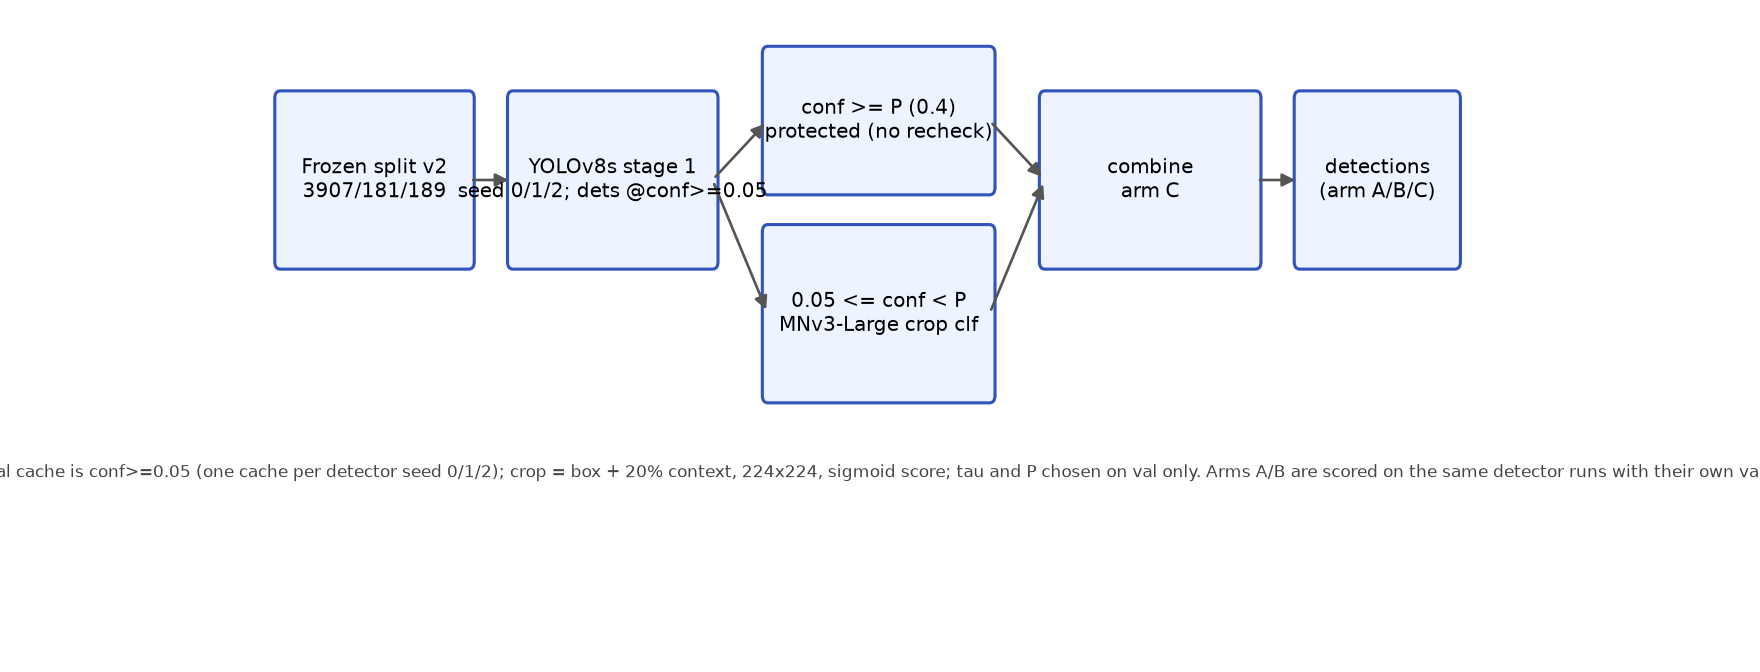
\includegraphics[width=0.88\linewidth]{figs/pipeline.png}
\caption{The two-stage pipeline as data flow. The detector proposes at a low
confidence ($0.05$); a proposal either bypasses the classifier when its detector
confidence is at least the protection threshold $P$, or is scored by the
MobileNetV3-Large crop classifier and compared against $\tau$. Both $P$ and
$\tau$ are chosen on validation. Arms A and B are the same detector run scored by
a single confidence, so the schematic differs between arms only in where the
final comparison happens, not in the features computed.}
\label{fig:pipeline}
\end{figure*}

\subsection{Statistics}

All test comparisons use the same $189$ images, so we resample images, not
detections. For a paired comparison between two arms we draw $5{,}000$ bootstrap
replicates of the image set \citep{efron1993bootstrap} and report the $95\%$
percentile interval of the difference. For single-arm uncertainty we additionally
report a source-cluster bootstrap over the three test sources, and a
leave-one-source-out analysis; with three clusters these intervals are wide by
construction, and we present them as such rather than as precise estimates.
Image-level agreement uses Cohen's $\kappa$ \citep{cohen1960kappa} alongside
balanced accuracy, because the test set has only $5$ negative images and raw
accuracy is dominated by the positive class.

\subsection{Attribution audit}

We compute Grad-CAM \citep{selvaraju2017gradcam} on the neck feature maps feeding
the detection head, targeting the top pre-NMS class score, and on the last
convolutional block of the classifier. Because the top pre-NMS anchor usually
sits on the stride-8 head, the largest stride with a non-zero gradient is used;
this deviates from the common stride-32 choice and is documented with the code.
We report four quantities: the share of CAM energy inside the ground-truth box
(and its enrichment over the box's area share), whether the CAM peak falls inside
the box, the drop in detection score when the box is masked versus when a
matched background region is masked, and a head-to-head comparison of detector
and classifier saliency on the same crops. Every sentence about these numbers is
phrased as evidence about \emph{where the model looked}, never about whether the
prediction is correct.

\section{Experimental Protocol and Reproducibility}
\label{sec:protocol}

\paragraph{Frozen rules.} Five rules governed every run, and we report violations
as well as compliance. (i) Thresholds are chosen on validation only. (ii) Every
evaluation that touches test is logged, numbered, and justified in advance.
(iii) Every number in this paper is produced by a committed script reading a
committed JSON or CSV. (iv) The original dataset and the pre-audit runs are never
modified. (v) Test labels are corrected only when objectively wrong, with
before/after numbers reported.

\paragraph{Test-touch accounting.} The full log contains $18$ numbered touches.
Four are large: the seed-0 frozen-protocol detector evaluation, the seed-0 and
seed-1/2 two-stage evaluations, and the corrected detector-aligned two-stage
re-scoring. The remainder are the per-seed detector evaluations, the MNv3
baseline evaluations, and the Grad-CAM passes, each sanctioned by the protocol
before execution. We also disclose a deviation: the upstream training script
auto-evaluates test at confidence $0.25$ at the end of training, and this
behaviour could not be disabled by flag. It is recorded as D017. No threshold,
checkpoint, or architecture choice references those numbers; they appear in no
table here. The frozen-protocol evaluation is a separate, single pass.

\paragraph{Correction we had to make.} An earlier version of the three-seed
two-stage result reused the seed-0 detector for all three seeds, producing a
tight mean of $0.879 \pm 0.018$. The arms A and B records were byte-identical
across seeds, which is the tell. Re-running the pipeline with each seed's own
detector gives $0.894 / 0.825 / 0.724$ and a standard deviation of $0.086$. The
tight interval was an artifact of a shared component. We report the corrected
numbers throughout and flag the earlier figure as withdrawn.

\paragraph{Compute.} All training and evaluation ran on one NVIDIA RTX~4070
Laptop GPU with $8$\,GB of memory, under Windows, within an approved budget of
roughly $30$ GPU-hours. Detector training took $50$--$85$ minutes per seed;
the second-stage classifier $30$ epochs per run; the ablation matrix five
classifier retrains. Evaluation uses $640\times640$ input, NMS IoU $0.7$,
\texttt{max\_det} $300$, FP32, no test-time augmentation. Latency figures are PC
GPU FP32 medians over $50$ repetitions after $10$ warm-up iterations, and are
\emph{not} edge-device numbers; no Jetson or TensorRT measurement was performed.

\paragraph{What the budget forbade.} We did not train YOLOv8m or YOLOv8l on the
clean split, did not evaluate a second detector family (RT-DETR or Faster
R-CNN), did not run grouped cross-validation, did not re-mine hard negatives on
data the detector had not seen, and did not retrain after the test-label
correction. Each omission is a real limitation and is listed in
Section~\ref{sec:limitations}. We prefer to name them than to let a single-seed
or single-family result stand in for a claim it cannot support.

\paragraph{Artifacts.} The repository contains the code, the six detector
checkpoints (three seeds, ONNX included), the three stage-2 checkpoints, the
frozen split manifest and its digest, all evaluation JSONs, the generated tables,
and the figures. Regenerating the tables requires no GPU and no dataset: the
committed JSONs are sufficient, and the table script fails loudly if a required
field is missing rather than silently substituting a value.

\section{Results}
\label{sec:results}

\subsection{Size sweep: mAP saturates, the operating point does not}
\label{sec:size}

Table~\ref{tab:size} reports both depths. The mAP columns are almost flat:
$0.977 \pm 0.003$ for \texttt{yolov8s} over three seeds and $0.979$ for
\texttt{yolov8n} at one seed. On validation the gap is larger
($0.954$ vs.\ $0.932$), which means we cannot claim the smaller model is better
on this evidence: the difference is inside the seed spread of the larger model,
and a single-seed estimate on $189$ test images cannot resolve it. The defensible
reading is that mAP$_{50}$ cannot distinguish the two detectors.

\begin{table}[t]
\centering
\small
\caption{Size sweep on the frozen test split. \texttt{s} is mean $\pm$ std over
seeds $0/1/2$; \texttt{n} is seed $0$ only and therefore carries no interval.
``OP'' is the validation-chosen recall-first operating point
($R\ge0.97$ on validation), applied unchanged to test. Latency is PC GPU FP32,
$640\times640$, median of $50$ runs.}
\label{tab:size}
\scriptsize
\setlength{\tabcolsep}{3pt}
\begin{tabular}{lrrrrrrrrr}
\toprule
model & params & GFLOPs & MB & ms & val mAP$_{50}$ & test mAP$_{50}$ & $R$ & $P$ & FP/img \\
\midrule
yolov8s & 11.1\,M & 28.6 & 21.5 & 6.5 & $0.9544\pm0.0027$ & $0.9768\pm0.0034$ & $0.9763\pm0.0040$ & $0.5157\pm0.2180$ & $1.510\pm1.009$ \\
yolov8n & 3.0\,M & 8.2 & 6.0 & 6.9 & 0.9322 & 0.9787 & 0.9842 & 0.1686 & 6.497 \\
\bottomrule
\end{tabular}
\end{table}

The operating-point columns are not flat at all. At the recall-first point the
smaller detector emits \fpn\ false positives per image against \fps\ for the
larger one---a $4.3\times$ difference, and notice the direction: the model with
fewer parameters is \emph{worse} at deployment while being equal or better on
mAP. Its precision at that point is $0.169$ against $0.516$. The mAP$_{50}$ of
$0.979$ is earned by ranking, not by calibration, and at a fixed high-recall
threshold the ranking advantage evaporates.

This is the paper's central empirical claim, and it is a claim about evaluation.
A benchmark that reports only mAP$_{50}$ would rank \texttt{yolov8n} first and
recommend it for a $8.2$\,GFLOP budget; a deployment engineer would get a
detector emitting four times as many alarms per frame. We note one more
inconvenient detail: measured latency does not favour the smaller model
($6.9$ vs.\ $6.5$\,ms), because at this size the fixed per-image overhead
dominates. The GFLOP and parameter savings are real, the wall-clock saving on
this hardware is not. Reporting FLOPs as a proxy for latency is another summary
statistic that fails to transfer.

\begin{table}[t]
\centering
\small
\caption{Per-seed operating points for \texttt{yolov8s}. The threshold chosen on
validation varies by an order of magnitude across seeds ($0.01$ to $0.21$) and
so does the resulting precision. Test mAP barely moves.}
\label{tab:seed}
\begin{tabular}{lcccccc}
\toprule
seed & val conf & test mAP$_{50}$ & box $P$ & box $R$ & FP/img & image $R$ [95\% CI] \\
\midrule
0 & 0.020 & 0.9741 & 0.427 & 0.976 & 1.751 & 1.000 [0.980, 1.000] \\
1 & 0.010 & 0.9807 & 0.356 & 0.980 & 2.376 & 0.995 [0.970, 0.999] \\
2 & 0.210 & 0.9756 & 0.764 & 0.972 & 0.402 & 0.984 [0.953, 0.994] \\
\bottomrule
\end{tabular}
\end{table}

Table~\ref{tab:seed} exposes the mechanism. The three seeds reach nearly identical
test mAP ($0.974$--$0.981$) and nearly identical recall ($0.972$--$0.980$), but
the validation procedure selects thresholds of $0.02$, $0.01$, and $0.21$,
producing precisions of $0.427$, $0.356$, and $0.764$. Seed 2 is eight to ten
times more conservative at the same mAP. Any claim about ``the model's precision''
that pools these seeds is a claim about the threshold-selection procedure, not
about the detector. We therefore report per-seed values wherever precision or
FP/image is the quantity of interest, and treat the three-seed mean as a summary
of protocol variance rather than of model quality.

\subsection{Where the variance lives: source structure}
\label{sec:persource}

The source-cluster bootstrap makes the same point from a different direction. For
seed 0, resampling the three test sources gives $P \in [0.195, 0.874]$,
$R \in [0.948, 1.000]$, and $\mathrm{FP/img} \in [0.139, 30.1]$. With three
clusters these intervals are honest but almost uninformative; the
leave-one-source-out analysis is more legible. Removing \texttt{Jan\_lwir}---the
ten images that generate most of the false alarms---raises seed-0 precision from
$0.427$ to $0.853$ and drops FP/image from $1.75$ to $0.17$. Removing
\texttt{ds0} does the opposite: precision falls to $0.246$ and FP/image rises to
$8.16$, because the remaining \texttt{Jan} false positives are divided by far
fewer true positives.

Table~\ref{tab:persource} gives the direct decomposition. Ten \texttt{Jan} test
images account for $301$ of the $331$ false positives emitted by arm A---$91\%$
of all false alarms come from $5\%$ of the images. The two-stage arm reduces that
to $21$, and reduces total FP/image from $1.75$ to $0.15$, but it also costs
recall on that source ($0.948 \to 0.909$). The honest summary is that the
aggregate metric is dominated by a source that is over-represented in boxes and
under-represented in images, and that any intervention which suppresses
\texttt{Jan} false alarms will look like a large aggregate gain while being a
modest, source-specific change.

\begin{table}[t]
\centering
\small
\caption{Per-source test results for seeds 0, arm A (YOLO at deploy threshold)
and arm C (two-stage). All $331$ arm-A false positives come from three sources;
$301$ of them from ten \texttt{Jan} images.}
\label{tab:persource}
\begin{tabular}{llrrrrrr}
\toprule
arm & source & images & TP & FP & $P$ & $R$ & FP/img \\
\midrule
A & Jan\_lwir & 10 & 73 & 301 & 0.195 & 0.948 & 30.100 \\
A & ds0 & 151 & 146 & 21 & 0.874 & 0.986 & 0.139 \\
A & ds1 & 28 & 28 & 9 & 0.757 & 1.000 & 0.321 \\
A & all & 189 & 247 & 331 & 0.427 & 0.976 & 1.751 \\
\midrule
C & Jan\_lwir & 10 & 70 & 21 & 0.769 & 0.909 & 2.100 \\
C & ds0 & 151 & 146 & 4 & 0.973 & 0.986 & 0.026 \\
C & ds1 & 28 & 28 & 4 & 0.875 & 1.000 & 0.143 \\
C & all & 189 & 244 & 29 & 0.894 & 0.964 & 0.153 \\
\bottomrule
\end{tabular}
\end{table}

We flag a confound: \texttt{Jan} and \texttt{May} are the sources whose filenames
claim thermal imagery but whose pixels are colour photographs with marker pins
(Section~\ref{sec:data}). If a marker cue is present, \texttt{Jan} false alarms
may be marker detections rather than mine detections, and the second stage may be
suppressing markers rather than terrain. Our twelve-crop check did not find a
consistent marker near test mines, but the confound cannot be excluded from this
data, and it is one reason we do not claim the two-stage gain is about mines.

\subsection{Image level}
\label{sec:imagelevel}

Table~\ref{tab:imagelevel} asks a coarser question: does the image contain a mine
at all? The frozen-feature MobileNetV3 baseline is degenerate on this task. Its
stage-A variant reaches $0.974$ accuracy but balanced accuracy $0.500$ and
$\kappa = 0.000$: it calls every image positive, which is correct for $184$ of
$189$ images and useless for triage. Fine-tuning the last layers (stage B) lifts
balanced accuracy to $0.562 \pm 0.056$ and $\kappa$ to $0.156 \pm 0.148$; still
weak, and with a standard deviation across three seeds that spans zero agreement.

The detector is a different regime. At its deploy threshold it reaches balanced
accuracy $0.830 \pm 0.115$ and $\kappa = 0.677 \pm 0.199$; at $\mathrm{OP}_{95}$
it reaches $0.993 \pm 0.002$ and $\kappa = 0.784 \pm 0.038$. The two-stage arm
reaches $0.962 \pm 0.059$ and $\kappa = 0.818 \pm 0.094$. The high variance of the
deploy row is the threshold-transfer problem again: one seed's validation choice
produces a conservative test operating point and another's does not.

\begin{table}[t]
\centering
\small
\caption{Image-level decisions on test. MNv3 A is seed 0; A+B is mean $\pm$ std
over three seeds; YOLO and two-stage rows are mean $\pm$ std over three detector
seeds. Balanced accuracy and $\kappa$ are the meaningful columns given only five
negative images.}
\label{tab:imagelevel}
\begin{tabular}{lccccc}
\toprule
system & accuracy & balanced acc & precision & recall & $\kappa$ \\
\midrule
MNv3 A (thr 0.5) & 0.974 & 0.500 & 0.974 & 1.000 & 0.000 \\
MNv3 A (recall-first) & 0.968 & 0.497 & 0.973 & 0.995 & $-0.009$ \\
MNv3 A+B (thr 0.5) & $0.974\pm0.000$ & $0.500\pm0.000$ & $0.974\pm0.000$ & $1.000\pm0.000$ & $0.000\pm0.000$ \\
MNv3 A+B (recall-first) & $0.968\pm0.005$ & $0.562\pm0.056$ & $0.977\pm0.003$ & $0.991\pm0.006$ & $0.156\pm0.148$ \\
YOLO deploy & $0.984\pm0.009$ & $0.830\pm0.115$ & $0.991\pm0.006$ & $0.993\pm0.008$ & $0.677\pm0.199$ \\
YOLO $\mathrm{OP}_{95}$ & $0.986\pm0.003$ & $0.993\pm0.002$ & $1.000\pm0.000$ & $0.986\pm0.003$ & $0.784\pm0.038$ \\
Two-stage (arm C) & $0.989\pm0.005$ & $0.962\pm0.059$ & $0.998\pm0.003$ & $0.991\pm0.003$ & $0.818\pm0.094$ \\
\bottomrule
\end{tabular}
\end{table}

The MNv3 result is worth stating plainly because it is a negative result about a
standard baseline: a classifier that achieves $97.4\%$ accuracy has learned
nothing about the task. Accuracy on a $97.4\%$-positive test set is not evidence.
We keep the row to make the point, and we use the classifier only as a
\emph{second stage} over detector crops, where the proposal mechanism supplies
the localisation the image-level baseline lacks.

\subsection{Two-stage: per-seed, not pooled}
\label{sec:twostage}

Table~\ref{tab:twostage} is the result we most want to be read carefully. Pooled
over seeds, arm C looks like a clean win: precision $0.814 \pm 0.086$ versus
$0.734 \pm 0.050$ for the recall-matched baseline, FP/image $0.31$ versus $0.48$.
The per-seed structure is not a clean win.

\begin{table}[t]
\centering
\small
\caption{Two-stage ablation on test, mean $\pm$ std over detector seeds
$0/1/2$ (arm thresholds in the second column). Arm A is YOLO at its deploy
threshold; B is YOLO at the confidence matching arm A's validation recall; C adds
the classifier with protection $P=0.4$.}
\label{tab:twostage}
\setlength{\tabcolsep}{3.5pt}
\begin{tabular}{llccccc}
\toprule
arm & conf / $\tau$ (s0/s1/s2) & $P$ & $R$ & $F_2$ & FP/img & image $R$ \\
\midrule
A & 0.02 / 0.01 / 0.21 & $0.516\pm0.218$ & $0.976\pm0.004$ & $0.808\pm0.102$ & $1.510\pm1.009$ & $0.993\pm0.008$ \\
B & 0.125 / 0.06 / 0.21 & $0.734\pm0.050$ & $0.974\pm0.002$ & $0.913\pm0.014$ & $0.478\pm0.127$ & $0.989\pm0.005$ \\
C & $\tau$ 0.27 / 0.23 / 0.22 & $0.814\pm0.086$ & $0.968\pm0.004$ & $0.932\pm0.020$ & $0.309\pm0.174$ & $0.991\pm0.003$ \\
\bottomrule
\end{tabular}
\end{table}

Paired bootstrap, one row per detector seed (Table~\ref{tab:cb}).

\begin{table}[t]
\centering
\small
\caption{Paired bootstrap for arm C minus arm B, computed separately per detector
seed ($5{,}000$ resamples over the $189$ test images). An interval spanning zero
means the arms are indistinguishable at that seed.}
\label{tab:cb}
\setlength{\tabcolsep}{5pt}
\begin{tabular}{lccc}
\toprule
detector seed & $\Delta P$ [95\% CI] & $\Delta$FP/img [95\% CI] & $\Delta R$ [95\% CI] \\
\midrule
0 & $+0.128\ [0.065, 0.186]$ & $-0.2529\ [-0.4603, -0.0952]$ & $-0.0079\ [-0.0195, 0.0000]$ \\
1 & $+0.144\ [0.096, 0.181]$ & $-0.3466\ [-0.5979, -0.1587]$ & $-0.0079\ [-0.0195, 0.0000]$ \\
2 & $-0.037\ [-0.077, 0.013]$ & $+0.0927\ [-0.0212, 0.2275]$ & $+0.0001\ [-0.0199, 0.0166]$ \\
\bottomrule
\end{tabular}
\end{table}

Seeds 0 and 1 gain precision and lose a small, bounded amount of recall; the
precision and false-positive intervals exclude zero. Seed 2 moves the other way:
the precision point estimate is negative and every interval spans zero, so the
two-stage pipeline does not help that detector.

The mechanism is visible in the arm-A confidences. At seed 2 the validation
procedure selects $0.21$ for both the deploy and the matched-recall arms, so arms
A and B coincide: the baseline is already operating at a well-transferred
threshold, and the classifier has no error mass to remove. At seeds 0 and 1 the
validation threshold is $0.02$ and $0.01$, both of which transfer badly to test
and produce $1.75$ and $2.38$ false positives per image. The classifier repairs
that specific failure. It is not improving localisation; it is compensating for a
threshold that did not generalise.

Two consequences follow, and both cut against the headline. First, the two-stage
effect is not a stable property of the architecture; it is conditional on the
baseline being badly thresholded. Any paper reporting the three-seed mean without
this decomposition is reporting a protocol artifact. Second, if one is allowed to
tune the single-stage threshold on validation with the same freedom, the
classifier loses under a max-$F_2$ objective. For seed 0, a YOLO confidence of
$0.52$ on validation gives test $P = 0.976$, $R = 0.949$, $\mathrm{FP/img} = 0.032$,
against $P = 0.945$, $R = 0.957$, $\mathrm{FP/img} = 0.074$ for the best
max-$F_2$ two-stage configuration. The single stage is $3.1$ points better in
precision and emits less than half the false alarms, at $0.8$ points less recall.
The defensible role for the classifier is therefore narrower than the aggregate
table suggests: the strict high-recall regime ($R \ge 0.96$) and
terrain-nuisance rejection. It is not a general-purpose improvement, and we say
so.

\begin{figure}[t]
\centering
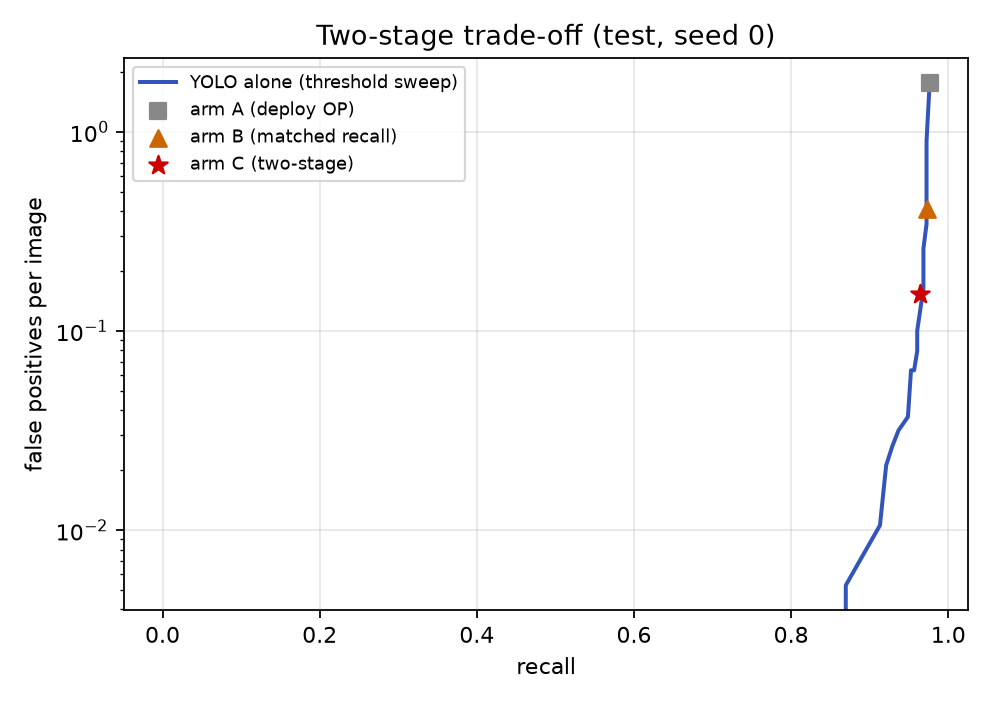
\includegraphics[width=0.78\linewidth]{figs/fp_recall_tradeoff.png}
\caption{False positives per image against recall for the single-stage and
two-stage arms (seed 0). The classifier's advantage is concentrated at high
recall; at moderate recall a tuned single-stage threshold is better. Curves are
drawn from the same frozen test records used in Table~\ref{tab:twostage}.}
\label{fig:tradeoff}
\end{figure}

\subsection{Second-stage ablations}
\label{sec:ablation}

Five variants isolate the recipe (Table~\ref{tab:ablation}). Removing hard
negatives is the largest single degradation
($\Delta P = -0.056\ [-0.084, -0.028]$), which is unsurprising given that the
negatives are detector false positives rather than random background. Removing
context padding ($0.0$) costs $0.027$ precision, and doubling it ($0.4$) costs
$0.025$: the $20\%$ margin is a genuine optimum rather than a monotone knob.
Reducing crop resolution to $160$ \emph{improves} precision by $0.017$ with an
interval that touches zero $[0.000, 0.036]$, a difference we do not claim.
Doubling to $320$ costs $0.025$. All intervals are paired image bootstraps
against the baseline on the same test images.

\begin{table}[t]
\centering
\small
\caption{Stage-2 ablations at the validation-chosen recall-safe rule, detector
seed 0. $\Delta P$ is a paired image bootstrap against the baseline; an interval
spanning zero means indistinguishable.}
\label{tab:ablation}
\begin{tabular}{lccccccc}
\toprule
variant & pad & crop & hard neg. & $\tau$ & $P$ & FP/img & $\Delta P$ [95\% CI] \\
\midrule
baseline & 0.2 & 224 & yes & 0.27 & 0.894 & 0.153 & reference \\
crop 160 & 0.2 & 160 & yes & 0.43 & 0.911 & 0.127 & $+0.017\ [0.000, 0.036]$ \\
crop 320 & 0.2 & 320 & yes & 0.08 & 0.868 & 0.196 & $-0.025\ [-0.049, -0.006]$ \\
no hard neg. & 0.2 & 224 & no & 0.35 & 0.837 & 0.254 & $-0.056\ [-0.084, -0.028]$ \\
pad 0.0 & 0.0 & 224 & yes & 0.16 & 0.866 & 0.201 & $-0.027\ [-0.043, -0.011]$ \\
pad 0.4 & 0.4 & 224 & yes & 0.25 & 0.868 & 0.196 & $-0.025\ [-0.042, -0.011]$ \\
\bottomrule
\end{tabular}
\end{table}

\subsection{Grad-CAM: evidence, not correctness}
\label{sec:gradcam}

We use attribution as a falsification tool and report what it shows, including
where it is uninformative. On $244$ true-positive detections, the median share of
CAM energy inside the ground-truth box is $0.939$ (mean $0.690$, first quartile
$0.0002$, third quartile $0.996$). Median enrichment over the box's area share is
$58.2\times$; the peak falls inside the box for $73.0\%$ of detections. The
bimodality is important: the distribution is not centred on a high value, it is
split between detections whose evidence is almost entirely on the object and
detections whose evidence is almost entirely elsewhere. The second group is
where the detector is right for the wrong reason.

Deletion tests confirm the direction. Masking the ground-truth box lowers the
detection score by $0.739$ on average ($n=182$); masking a matched background
region lowers it by $0.0015$. The detector's score depends on the object region,
as it should.

The head-to-head comparison is the cautionary result. On images where both the
detector and the image-level classifier are correct, detector enrichment has
median $86.0\times$ and the MobileNetV3 baseline has median $1.82\times$; the
paired difference is $+147.0\ [125.4, 170.0]$ in favour of the detector. On
detector crops, the stage-2 classifier reaches only $2.13\times$. The classifier
that achieves $97.4\%$ image-level accuracy is not looking at the object in any
localised sense; it is exploiting context. That does not make its decisions wrong
on this test set, but it explains why fine-tuning it adds so little precision and
why its gains vanish when the baseline threshold is already good.

\begin{figure}[t]
\centering
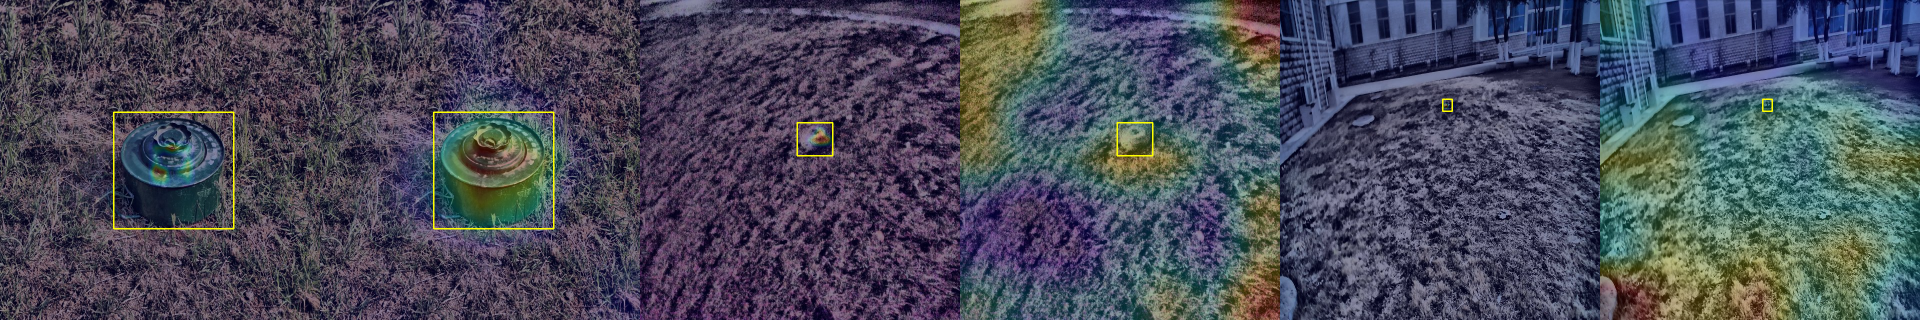
\includegraphics[width=0.95\linewidth]{figs/gradcam_example_grid.png}
\caption{Grad-CAM on detector crops (top) and image-level classifier (bottom).
The detector's evidence is object-localised; the classifier's is diffuse. This is
a statement about where each model looks, not about whether either prediction is
correct.}
\label{fig:gradcam}
\end{figure}

A paste-and-remove test probes the same question behaviourally. Pasting a mine
crop into a background yields detection at $0.650$ under the deploy confidence
and $0.630$ at the matched-recall confidence, against $0.976$ recall on original
images; inpainting a mine out of an image makes it disappear in $100$ of $100$
composites. The asymmetry is expected: synthetic pastes carry feathered edges and
scale mismatch, so the detector is being asked to fire on an object that looks
slightly wrong. We report the numbers as an upper bound on the paste setup's
realism, not as an estimate of the detector's sensitivity to context. The
zero-energy cases are more useful: exactly two test images had zero CAM energy in
the box, and both were the objectively wrong labels found in manual review. That
independent confirmation is the strongest evidence in this section that the
attribution pipeline is measuring something real.

Finally, the failure catalogue (Table~\ref{tab:failures}) is the qualitative
counterpart. Of $29$ reviewed false positives, $22$ are terrain texture; of $9$
false negatives, $5$ are camouflaged or low-contrast objects and $2$ are small.
The failure mass is where the deployment risk is, and it is not visible in any
aggregate score.

\begin{table}[t]
\centering
\small
\caption{Hand-reviewed failure categories at the arm-C deployment threshold
(seed 0). False positives are capped at $50$; $29$ were present.}
\label{tab:failures}
\begin{tabular}{lrr}
\toprule
category & FN & FP \\
\midrule
camouflaged or low contrast & 5 & 0 \\
small object & 2 & 0 \\
label error & 2 & 0 \\
terrain texture & 0 & 22 \\
low-light ground & 0 & 2 \\
fence / structure edge & 0 & 2 \\
structure wall & 0 & 1 \\
sensor noise & 0 & 1 \\
tree trunk & 0 & 1 \\
\midrule
total & 9 & 29 \\
\bottomrule
\end{tabular}
\end{table}

\begin{figure}[t]
\centering
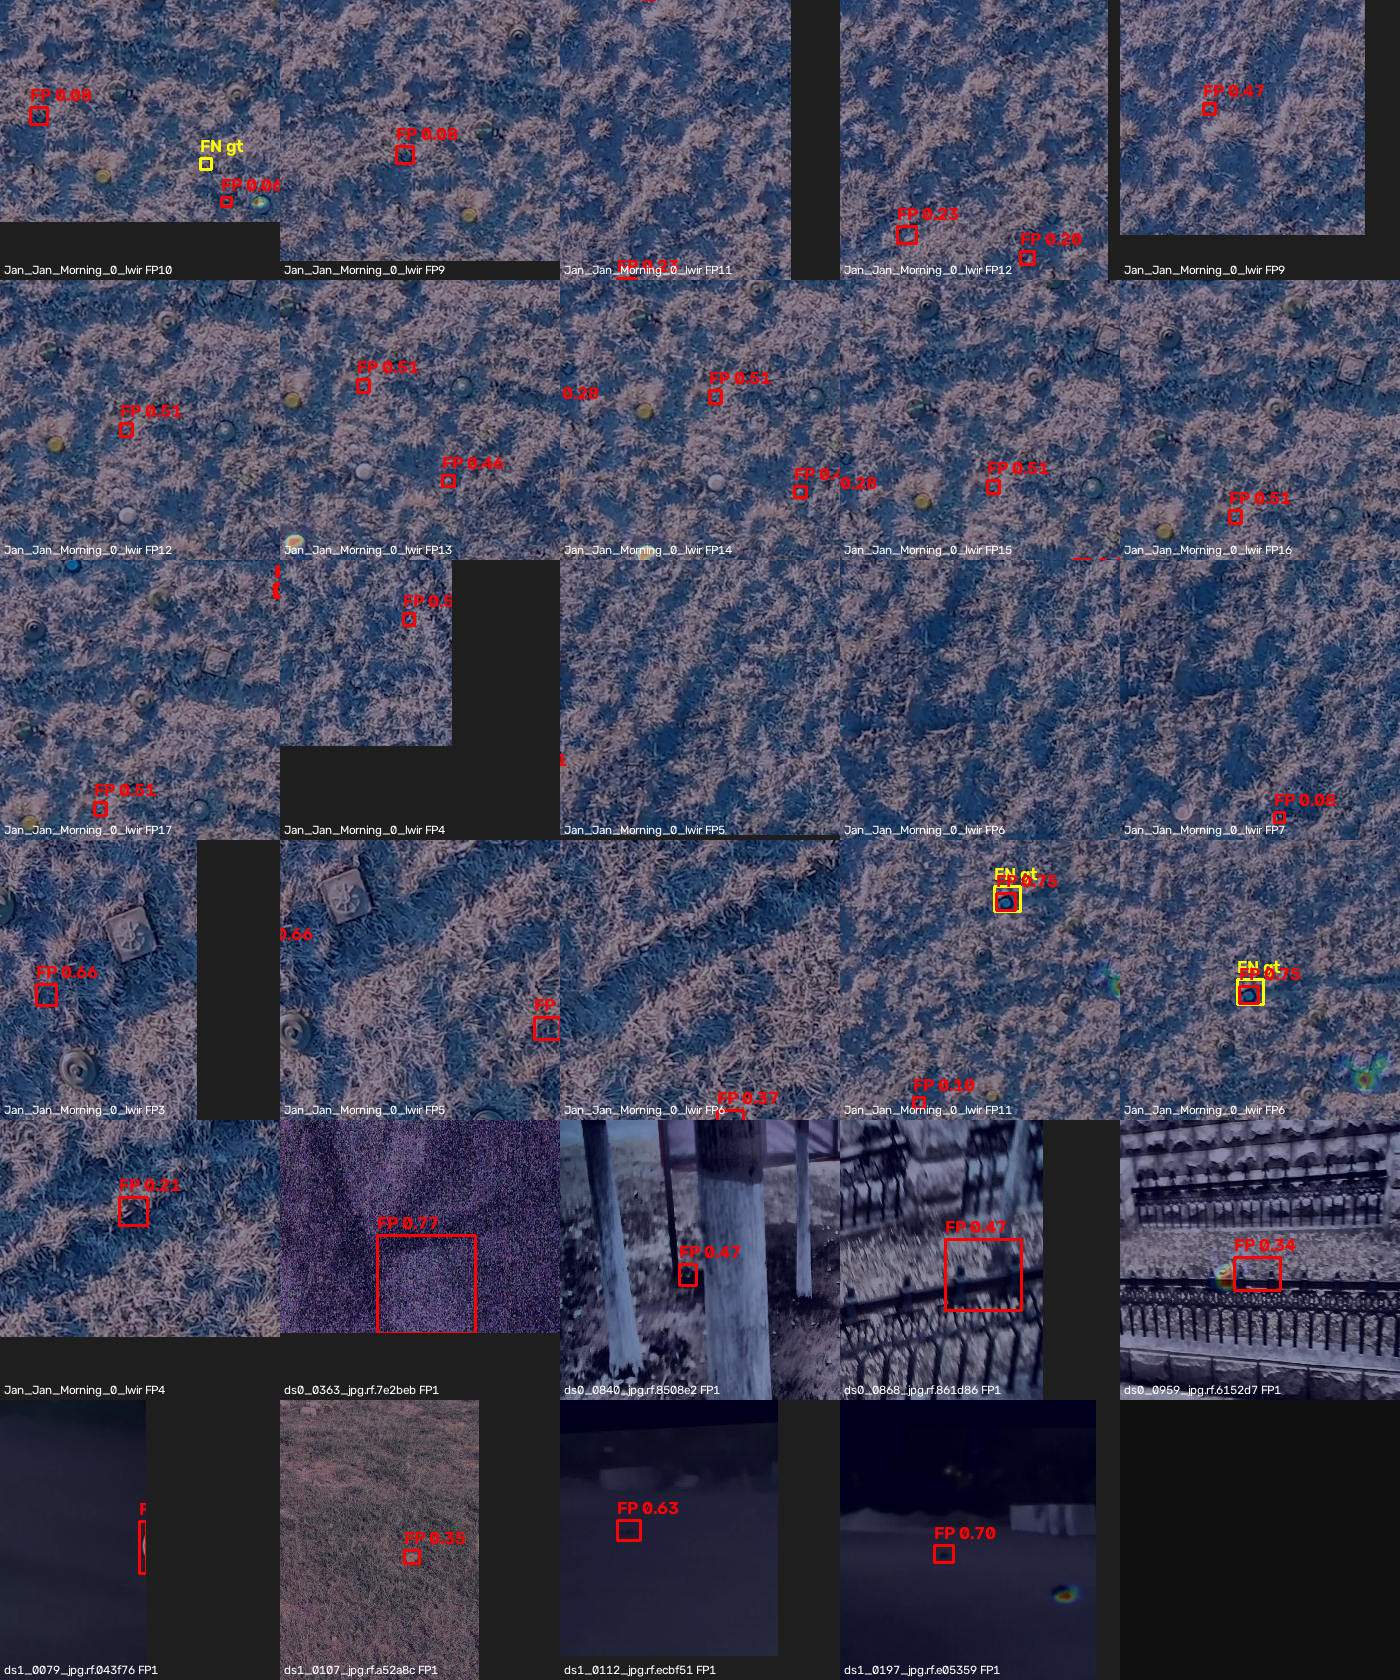
\includegraphics[width=0.62\linewidth]{figs/failure_gallery_fp.png}
\caption{Representative false positives. Terrain texture dominates; the
distinction between a mine-like disc and a rock or a patch of ground is the
failure mode that matters operationally.}
\label{fig:failures}
\end{figure}

\section{Discussion}
\label{sec:discussion}

\paragraph{Report the operating point, then the curve.} The size sweep is a
case study showing that mAP and deployment behaviour are different measurements.
Three \texttt{yolov8n} seeds and five \texttt{yolov8s} seeds are close on test
mAP ($0.979 \pm 0.003$ vs.\ $0.976 \pm 0.003$, intervals overlapping), but
validation mAP favors s by more than a seed standard deviation and the two
families differ by $6.2\times$ in false alarms at the recall-first point. The
result should motivate a threshold-rule sweep rather than a model ranking claim.
The mechanism is not mysterious: mAP integrates over confidence, and a model can
rank detections well while being badly calibrated near the threshold a user will
pick. The recommendation is concrete and cheap. Report, at minimum: the
validation procedure used to choose a threshold, the threshold itself for every
seed, and precision, recall, and false-positives-per-image at that threshold on
test. Report mAP as well, for comparability, but do not let it be the only row.

\paragraph{Threshold transfer is the hidden variable.} Our five seeds select
thresholds of $0.02$, $0.01$, $0.21$, $0.045$ and $0.125$ for the same
architecture, same data, same schedule. That is not a bug in the search; it is
what happens when a validation set has $181$ images and $7$ negatives. The
consequence is that ``model precision'' pooled over seeds is mostly a statement
about which threshold each seed happened to pick. This is consistent with the
two-stage result: the classifier looks valuable exactly where the threshold
transferred badly, and actively harmful where the selection rule chose a
near-inert configuration, but five seeds with shared components do not identify
that as a mechanism. Any ablation that changes a component downstream of a fragile
threshold will inherit that fragility, and a single pooled mean will hide it.

\paragraph{When is a second stage worth it?} On this evidence, narrowly. The
classifier is defensible if the requirement is recall $\ge 0.96$ with minimum
false alarms, and if the detector's threshold is known to be unreliable. It is
not defensible as a general precision improvement, because a tuned single-stage
threshold beats it at max-$F_2$, and its benefit disappears at the seed whose
threshold transferred well. The cost is real and it is not a rounding error:
$16.5 \pm 1.4$\,ms per image end to end against $6.5$\,ms for the single stage,
with $2.8 \pm 0.6$ crops scored per image and a 95th percentile of $5.3$
(Table~\ref{tab:cost}). For a pipeline that processes every frame of a flight,
that is a $2.5\times$ multiplier bought for a gain that is conditional on the
detector's threshold being unreliable. A deployment decision here is not
``which model is more accurate'' but ``how many false alarms is worth $2.5\times$
the frame budget'', and only the second question has an operational answer.

\paragraph{Leakage is worth measuring, not just fixing.} The contamination-free
comparison is a negative result, and we think negative results of this kind
should be routine. Fixing a split is good practice; quantifying what the fix
changed is what tells the reader whether the original numbers were wrong by
$0.002$ or by $0.2$. Here it is $0.0003$ on the comparable subset. We would not
have known that from the audit alone, and we would have been tempted to describe
the leak as catastrophic.

\paragraph{What the saliency audit bought.} Not much, and we say so rather than
dressing it up. On the $12$ multi-object test images the metric we used is not
even well defined, because a single per-image CAM is reused for every detection;
on the $172$ single-object images the detector's evidence is cleanly
object-localised (median energy share $0.98$, enrichment $\approx90\times$), which
is a statement about localisation, not about correctness. The image-level
baseline's low enrichment is partly a promise of the $20\%$ padding geometry
under which the ground-truth box occupies most of the crop, and the frozen
variant is degenerate on negatives. The audit's one useful output was as a
consistency check on two manually identified label errors. Attribution did not
prove any prediction correct, and the revised interpretation keeps it as a sanity
check rather than a mechanistic explanation.

\section{Limitations}
\label{sec:limitations}

\begin{enumerate}[leftmargin=1.4em,itemsep=2pt]
\item \textbf{Compute.} All results come from one $8$\,GB laptop GPU and roughly
$30$ GPU-hours. This single constraint explains most of the gaps below. We state
it once rather than repeating it as a caveat on every claim.
\item \textbf{One detector family, two depths on the clean split.} YOLOv8s
(five seeds) and YOLOv8n (three seeds). YOLOv8m was trained only on the old leaky
split and is therefore not comparable; we exclude it from the size sweep rather
than presenting a contaminated point.
\item \textbf{Small-model seed count, and shared components.} The \texttt{yolov8n}
row now carries an interval over three seeds, but its test mAP sits inside the
\texttt{yolov8s} interval, so the two are not distinguishable on that metric. The
five two-stage seeds are also not five independent systems. All five are
detector-aligned at evaluation time, each scoring its own stage-1 detections, but
seeds 0--2 train their classifier on a single crop set generated once from the
seed-0 detector, while seeds 3--4 generate their own crops. The stage-2 recipe is
held fixed throughout, and the stage-2 classifiers themselves are separately
trained (distinct checkpoints per seed). The effective replication is closer to
four.
\item \textbf{Unresolved checks.} We did not sweep recall targets and FP budgets
exhaustively, did not threshold-match the leaky and clean models, and did not
retrain after the label correction. The leak count rests on the operational
filter plus an embedding-neighbour check that agreed on all $99$ survivors but
cannot exclude a single missed near-duplicate; one candidate pair
(\texttt{ds1\_0054}/\texttt{ds1\_0111}) is reported in the run log as unconfirmed.
\item \textbf{Five negative test images.} Precision and FP/image are
high-variance; the source-cluster intervals span an order of magnitude. Point
estimates in tables are accompanied by intervals wherever the interval is
meaningful.
\item \textbf{Label correction without retraining.} Two test boxes were removed
from ground truth. We report both versions, but the model was not retrained on
corrected labels because no training-label errors were found.
\item \textbf{No grouped cross-validation.} A single frozen split was used, as
required by the protocol. Group-aware $k$-fold would give a better estimate of
split variance and was not affordable.
\item \textbf{No hard-negative re-mining on unseen data.} The stage-2 negatives
come from detector false positives on the training split, which is the correct
procedure but limits how novel the negatives are.
\item \textbf{Synthetic composites.} The paste-and-remove experiment uses
feathered, scale-mismatched composites. It is a probe, not a counterfactual.
\item \textbf{No on-device characterisation.} All latency numbers in
Table~\ref{tab:size} are PC GPU FP32 at $640\times640$. No edge measurement is
reported here, so we make no claim about Jetson throughput or energy. The
accompanying AeroShield deployment project does serve this same single-class
model on a Jetson Nano via TensorRT and exposes a per-run timing summary, so the
gap is an instrumentation task rather than a change of model.
\item \textbf{Source confound.} \texttt{Jan} and \texttt{May} are colour
photographs with marker pins, despite \texttt{lwir} in the filename. Marker
shortcuts cannot be fully excluded, and the source dominates aggregate false
alarms.
\item \textbf{No field validation and no buried-object claim.} This is a
benchmark on visible surface indicators. It says nothing about burial depth,
soil type, or detection probability in real clearance conditions.
\end{enumerate}

\section{Ethics and Dual Use}
\label{sec:ethics}

\paragraph{What this system can and cannot do.} The detector recognises visible
mine-like objects and surface indicators in downward-looking colour imagery. It
cannot detect a buried object, because the sensor cannot see one. It has not been
flown, field-tested, or validated against ground truth collected in a real
clearance operation. Nothing in this paper supports a statement about detection
probability in the field, and we do not make one. The correct description is a
computer-vision benchmark on a public, publicly derived image corpus.

\paragraph{Dual use.} The same capability that helps a clearance team prioritise
ground could help someone avoid marked hazards. We publish standard detection
metrics, an audit methodology, and trained weights; we publish no targeting
guidance, no geographic coordinates, and no operational deployment procedure.
The dual-use risk is real but generic to visible-object detection, and we judge
that the methodological contribution---how to audit a leaky split and why to
report operating points---outweighs it. We note that the weights are released
under AGPL-3.0, which requires derivative services to publish their source; this
is a licence choice, not an ethical safeguard.

\paragraph{The cost of the miss rate.} At the primary operating point the
two-stage arm recalls $0.964$ of annotated instances, which on this test set means
nine missed objects out of $253$. Those nine are analysed in
Table~\ref{tab:failures}: five are camouflaged or low-contrast, two are small
objects, and two are the objectively wrong labels removed under D023. A
pre-correction recall of $0.964$ reads as a good number in a table; after the
two label corrections, the corresponding value is $0.972$. In a clearance context it
means that roughly one in twenty-eight annotated objects is not flagged, and the
misses are concentrated in exactly the low-contrast cases where a human reviewer
is most likely to defer to the model. No metric in this paper should be read as
saying the system is safe to rely on.

\paragraph{Data ethics.} The corpus is derived from public dataset exports and
contains no human subjects, no personal data, and no imagery of identified
individuals. We did not collect new data. The original licences were not recorded
at download time; we therefore redistribute no images (Section~\ref{sec:data}).
Where figures include source imagery, they are reproduced for scholarly comment
at low resolution and are not a dataset release.

\paragraph{Reporting.} We report the results that weaken our own claims---the
seed-2 failure of the two-stage pipeline, the negative leakage result, the
degenerate image-level baseline, the tuned single-stage threshold that beats the
pipeline---in the main text rather than in an appendix. The reason is practical:
a reader who is deciding whether to trust the positive results needs to know how
the negative ones were handled.

\section{Availability and Licensing}
\label{sec:availability}

\paragraph{Code and artifacts.} Training, evaluation, auditing, Grad-CAM and
table-generation code are released with the paper, together with all evaluation
JSONs, the generated tables, and the figures. The frozen split manifest is
released as a CSV with the following SHA-256 digest:

\begin{center}\small\ttfamily
748322d62ace769445d0bd2363699097\\
0c7a5115a99c9344e139099c608c80de
\end{center}

\noindent No image, label file, or crop is redistributed; see
\texttt{DATA\_PROVENANCE.md} for the reason and for the exact source inventory.

\paragraph{Weights.} Three detector seeds are released, each with
\texttt{best.pt}, \texttt{last.pt} and an ONNX export, plus three stage-2
checkpoints and the original v1 run for reference, all with a SHA-256 manifest.
The seed-3/4 \texttt{yolov8s} and seed-0--2 \texttt{yolov8n} runs discussed in
Section~\ref{sec:results} were trained on the same frozen split under the same
schedule; their evaluation JSONs are committed so every number in this paper is
reproducible, but their weight files are not part of the released tree.
The detector checkpoints are derivative works of Ultralytics YOLOv8 and are
distributed under \textbf{AGPL-3.0}; the stage-2 checkpoints are fine-tuned
torchvision MobileNetV3-Large and are distributed under the same repository
licence for consistency. Third-party terms are stated in
\texttt{models/NOTICE.md}. The repository code and the audit artifacts are
AGPL-3.0.

\paragraph{Reproduction.} Regenerating every table requires no GPU and no
dataset: the committed JSONs are sufficient. The table script exits with an error
if a required field is absent rather than substituting a value, so a clean clone
either reproduces the tables in this paper or fails visibly.

\paragraph{Persistent identifier.} No DOI has been assigned at the time of this
draft. The manifest digest above is a content-level identifier; a Zenodo DOI and
exact release tag will be added to the camera-ready release.


\bibliographystyle{IEEEtranN}
\bibliography{refs}

\appendices
\section{Decision log (abridged)}
\label{app:decisions}

The project kept a numbered decision register. The entries that bear on claims in
this paper are reproduced here; the full register, with dates and rationale for
all $23$ entries, is in \texttt{DECISIONS.md}.

\begin{table*}[t]
\centering
\small
\caption{Abridged decision register. Entries omitted here concern file layout and
tooling rather than claims.}
\label{tab:decisions}
\setlength{\tabcolsep}{4pt}
\begin{tabular}{@{}p{0.055\linewidth}p{0.86\linewidth}@{}}
\toprule
ID & Decision and reason \\
\midrule
D010 & Reject the original split. $76$ cross-split base-name groups; $63.8\%$
of evaluation images with a pHash-$\le2$ training neighbour; augmentation before
splitting confirmed in the upstream scripts. \\
D011 & Image-level and FP/image metrics blocked until the test split contains
negatives. It contained zero. \\
D012 & \texttt{May}/\texttt{Jan} files are colour RGB with marker pins, not
thermal, despite the \texttt{lwir} filename. Keep and disclose (D016). \\
D014 & Operational leak definition: exact MD5, or base key, or same-source
pHash$\le2$ \emph{and} $32\times32$ RGB MSE $\le 900$. Manual review of all $146$
candidates sets the MSE cut (same-scene $\le 817$, texture $\ge 958.6$). \\
D015 & Freeze \texttt{landmine\_combined\_v2} at 3{,}907/181/189 with $30$ eval
leaks removed; manifest digest \texttt{748322d6\ldots c80de}; true leak rate
$0/370$. \\
D017 & Disclosed protocol deviation: the upstream training script auto-evaluates
test at confidence $0.25$. No selection uses those numbers; the frozen-protocol
evaluation is a separate single pass. \\
D018 & Accept early stopping at epoch $67/75$ (best $47$) for the pilot run;
retrain at batch $8$ for comparability (D019). The pilot is not a paper result. \\
D020 & Frozen-feature MNv3 is degenerate on negatives at every resolution and
batch size ($\kappa \approx 0$); only fine-tuning the last layers separates them.
Stage A rows retained as the mandated ablation. \\
D021 & Threshold rule: sweep protection $P$, choose the largest $\tau$ within
$0.5$ points of stage-1 validation recall, then minimise validation FP/image.
All seeds select $P=0.4$. \\
D022 & Grad-CAM flags images by energy in the union of all ground-truth boxes,
not per detection; per-detection rows were an instance-count artefact on
multi-mine frames. \\
D023 & Remove two objectively wrong test boxes (tree trunk, fence); report
before/after; do not retrain (no training-label errors found). \\
\bottomrule
\end{tabular}
\end{table*}

\section{Test-touch accounting}
\label{app:touches}

Eighteen numbered test touches were logged during the original run; a further
seven were logged during the extended analysis. Grouped by purpose:

\begin{table*}[t]
\centering
\small
\caption{Test-touch accounting, grouped by purpose.}
\label{tab:touches}
\begin{tabular}{@{}p{0.10\linewidth}p{0.34\linewidth}p{0.48\linewidth}@{}}
\toprule
touches & purpose & sanctioning rule \\
\midrule
\#1--\#2 & audit read-only passes & leakage audit reads labels only \\
\#3 & MNv3 baseline, seed 0 & Phase 4 protocol eval, val-chosen thresholds \\
\#4 & YOLO seed-0 frozen-protocol eval & the single protocol-governing eval \\
\#5 & MNv3 seeds 1--2 & Phase 4 protocol eval \\
\#6--\#8 & two-stage seeds 0--2 & Phase 5 protocol eval, val-frozen \\
\#9--\#12 & Grad-CAM E1--E6 & Phase 6, read-only attribution \\
\#13--\#14 & YOLO seeds 1--2 & Phase 3 per-seed protocol eval \\
\#15--\#16 & leaky baseline, v1 split and clean subset & extended analysis \\
\#17 & YOLOv8n size point & size ablation, val-chosen threshold \\
\#18 & corrected detector-aligned two-stage & re-score, no selection \\
\#19 & YOLOv8n seeds 1--2 and YOLOv8s seeds 3--4 & seed extension, val-chosen thresholds \\
\#20 & operating-point sweep, five seeds per size & re-read of committed detection records, no selection \\
\#21 & stratified Grad-CAM re-cut & read-only attribution, strata fixed in advance \\
\#22 & threshold-selection bootstrap & re-read; validates the val-only rule, chooses nothing \\
\#23 & five-seed stage-2 audit & pipeline rerun with each seed's own detector \\
\#24 & seed-3/4 two-stage pipeline & extended analysis, val-chosen configuration \\
\#25 & embedding near-duplicate check & read-only audit, no detector evaluated \\
\bottomrule
\end{tabular}
\end{table*}

Only touch \#4 could contaminate a claim, and it is the evaluation the paper's
detector numbers come from. Touch \#18 is a correction: the original seed-1/2
two-stage runs had reused the seed-0 detector, which we detected from
byte-identical arm-A/arm-B records and corrected by re-running with each seed's
own checkpoint. No threshold was re-chosen on test; the per-seed validation
selection was rerun for the corrected detector records. Touches \#19--\#24 repeat
the same protocol on additional seeds; none of them altered a rule, a threshold
grid, or a selection criterion after looking at test.

\section{Failure gallery and reproduction commands}
\label{app:repro}

The false-positive contact sheet is reproduced in Figure~\ref{fig:failures}. The
full false-negative gallery, the audit montages, the per-image predictions, and
the Grad-CAM heatmaps are in the repository under \texttt{paper\_results/}.

\begin{figure*}[t]
\begin{verbatim}
# tables T1-T6 and figures (no GPU, no dataset required)
python src/reporting/make_tables.py

# frozen-protocol evaluation of a checkpoint
python src/evaluation/phase3_eval.py --run <run_dir> --out <out_dir>

# two-stage pipeline with each detector seed
python src/pipeline/phase5_pipeline.py --yolo <seed_best.pt> \
    --cls <stage2_best.pt> --arm-a-conf <val_conf> --out <out_dir>

# statistical analysis, bootstrap and policy rules
python src/analysis/analysis_stats.py
\end{verbatim}
\end{figure*}

Environment: Python 3.11.9, Ultralytics 8.4.117, PyTorch 2.6.0+cu124,
torchvision 0.21.0+cu124, NVIDIA RTX~4070 Laptop (8\,GB). Evaluation at
$640\times640$, NMS IoU $0.7$, \texttt{max\_det} $300$, FP32, no TTA.


\end{document}
